\documentclass[11pt,letterpaper]{article}

% include figures
\usepackage{graphicx}
% get nice colors
\usepackage{xcolor}

% change default font to Palatino (looks nicer!)
\usepackage[latin1]{inputenc}
\usepackage{mathpazo}
\usepackage[T1]{fontenc}
% load some useful math symbols/fonts
\usepackage{latexsym,amsfonts,amsmath,amssymb,wasysym}
% be able to insert code
\usepackage{listings}

% comfort package to easily set margins
\usepackage[top=1in, bottom=1in, left=1in, right=1in]{geometry}

% spacing after a paragraph
\setlength{\parskip}{.15cm}
% indentation at the top of a new paragraph
\setlength{\parindent}{0.0cm}


\begin{document}

\begin{center}
\Large
Ay190 -- Worksheet 7\\
Daniel DeFelippis\\
Date: \today
\end{center}

%%
%%
%% I worked with Scott Barenfeld
%%
%% All python code can be found in the ws7 directory in my repository
%%
%%

\section{Measuring $\pi$ with an MC Experiment}

The principle behind this problem is fairly simple. We set the radius of a circle
equal to 1 and put it inside a square of side length 2. Then, using simple geometry,
$$ \pi = \frac{4n}{N} $$
where $N$ is the sample size of points and $n$ is the number of those points that
are inside both the circle and the square. 

We use the line of code
\lstinputlisting[language=Python, firstline=13, lastline=13]{ws7.1.py}
to choose the sample sizes. With this line, sample sizes N are chosen to be
evenly spaced on a logarithmic scale, from 10 to about 300,000. 

Plotting the error vs the $\log_{10}$ of the sample size, we see that larger 
sample sizes do produce more accurate answers.

\begin{figure}[bth]
\centering
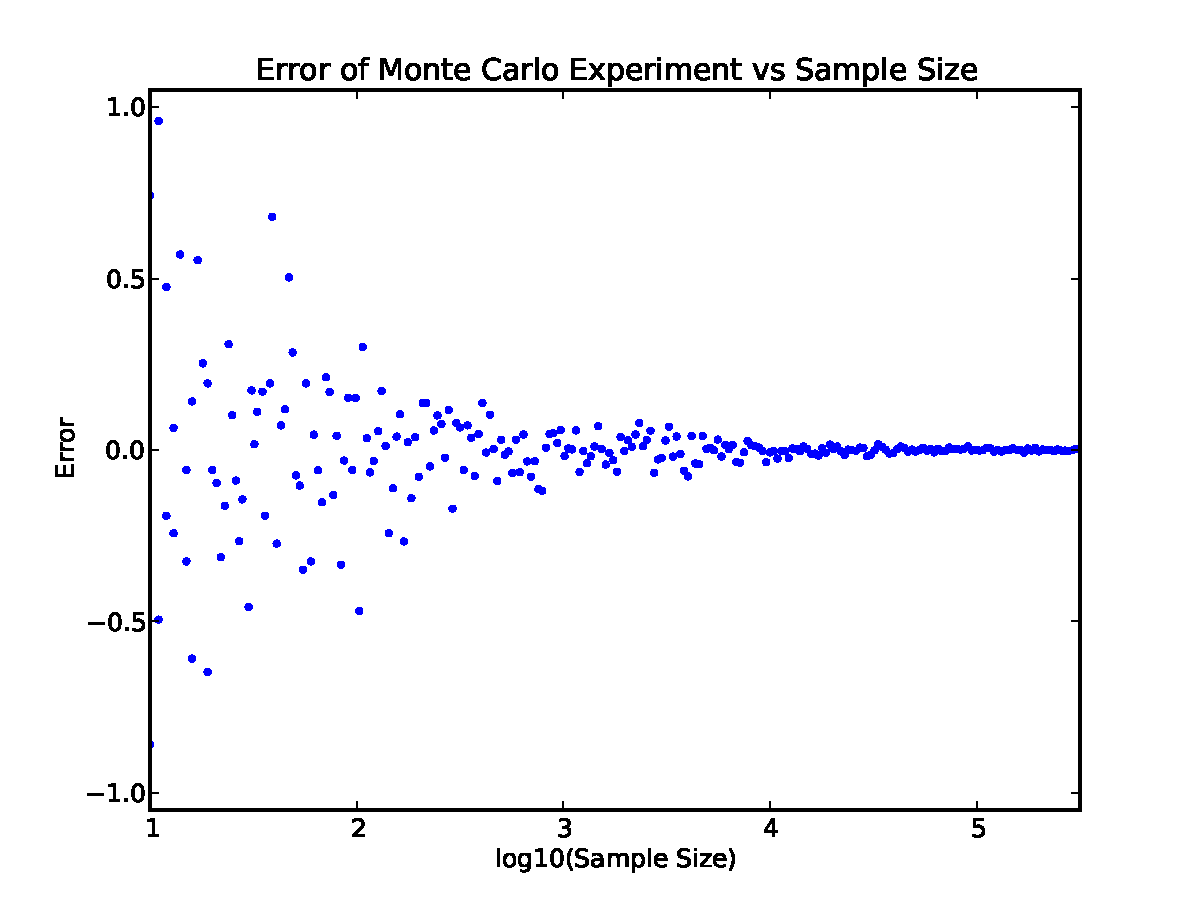
\includegraphics[width=0.85\textwidth]{pi_err_plot.pdf}
\caption{Error of MC calculation of $\pi$ vs $\log_{10} N$.}
\label{fig:piplot1}
\end{figure}

To really see how this error decreases, we plot a log-log graph of 
figure~\ref{fig:piplot1} above, making sure to take the absolute value of 
the error first.

\begin{figure}
\centering
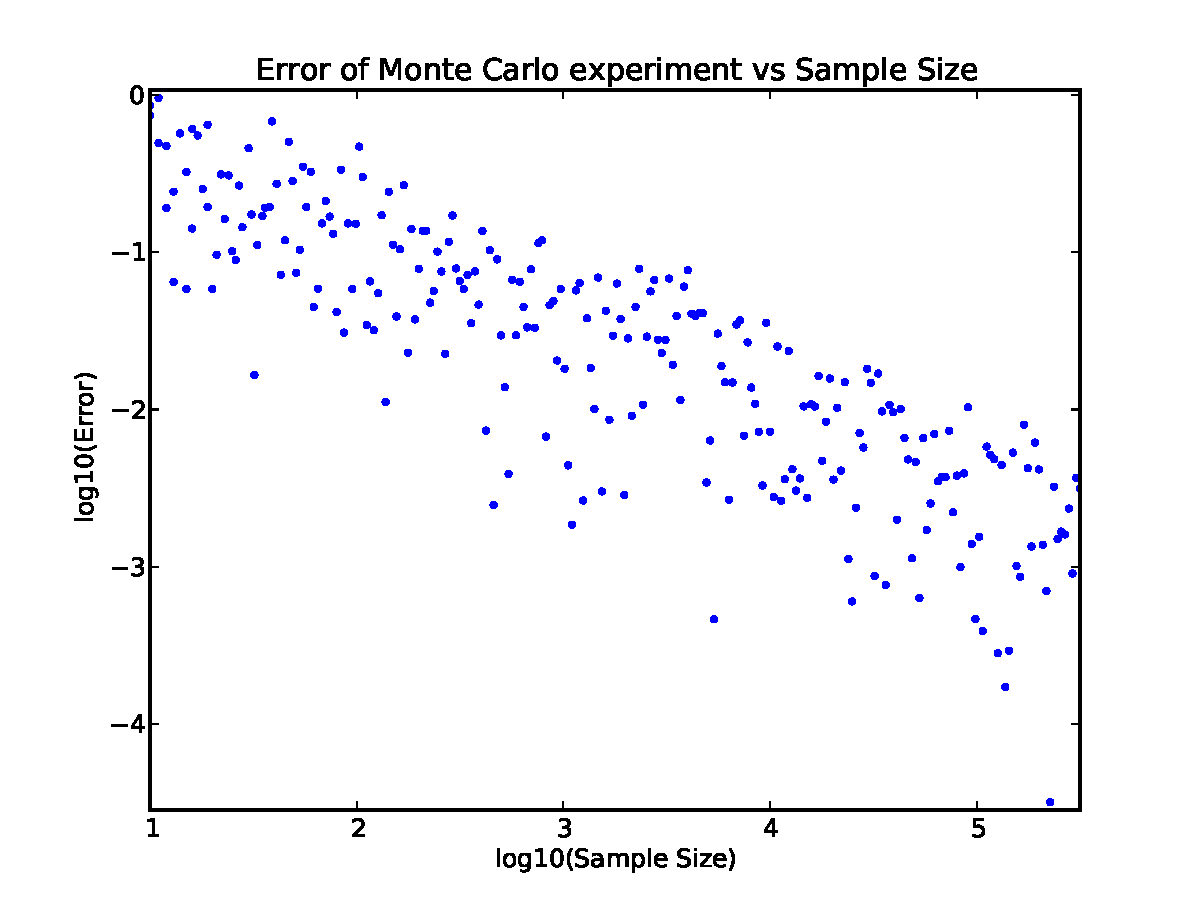
\includegraphics[width=0.85\textwidth]{pi_logerr_plot.pdf}
\caption{$\log_{10}$|error| vs $\log_{10} N$.}
\label{fig:piplot2}
\end{figure}  

From figure~\ref{fig:piplot2}, we see that the log of the error decreases 
as $-1/2$ times the log of the sample size, which means that, as
expected, this MC experiment converges as $1/\sqrt{N}$.

\section{The Birthday Paradox}

In order to solve this problem using an MC experiment, we need to create a 
list of random integers from 0 to 364, and then see if any number is repeated. 
We want to do this for different list sizes starting at 1 (for indexing 
convenience) and going up until we find at which size the probability of
having two numbers be the same is 50\%. 

We want a 2D probability array, with rows being a specific sample size 
and columns being a specific number of people. Coding this involves 
multiple "for" loops (over the different sample sizes, 
number of people, and values of the sample size), which means I couldn't 
get the same amount of data points as I did in problem 1. It also involves
the lines
\lstinputlisting[language=Python, firstline=38, lastline=39]{ws7.2.py}
The set() function returns an ordered list of a list you give it with the 
duplicates removed, so if the lengths of an array of N birthdays and an 
ordered array with duplicates removed aren't the same, then at least two 
people have the same birthday and we add 1 to our success counter.

Running the code, and manually looking at columns of the resulting probability 
array, we see that $\mathbf{N=23}$ is the number of people at which 
the probability crosses 50\%. Comparing this to the Wikipeda page for the Birthday
Paradox, we see that this answer is correct. From that page, we can compare 
our MC probabilities to the actual probability for $N = 23$ given by 
$$ P(23) = 1 - \frac{365!}{365^{23}(365-23)!} = 0.50729723432398544$$
to check convergence. First though, let's see why that formula for the probability
makes sense. 

\begin{figure}[bth]
\centering
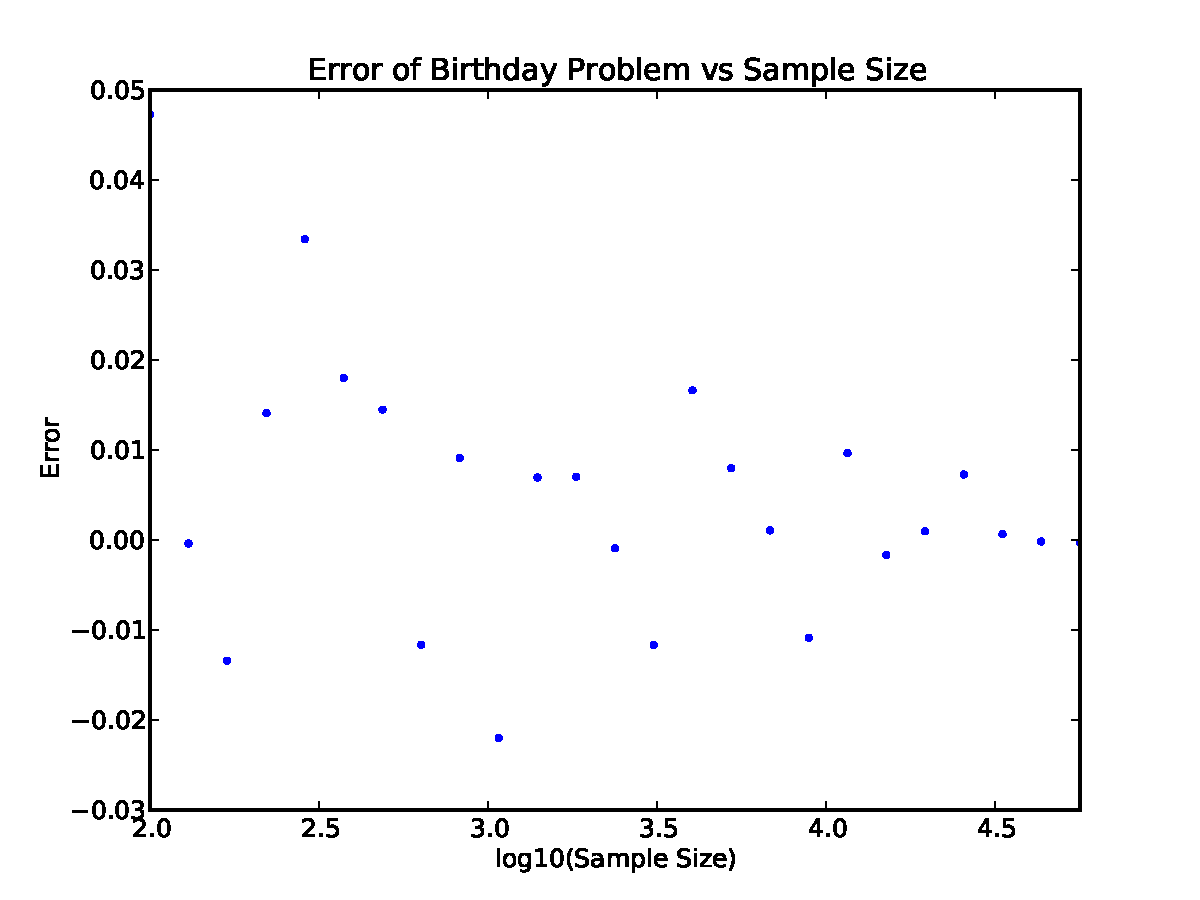
\includegraphics[width=0.8\textwidth]{birth_err_plot.pdf}
\caption{Error of MC Birthday probabilities ($N=23$) vs $\log_{10} N$.}
\label{fig:birthplot1}
\end{figure}

\begin{figure}
\centering
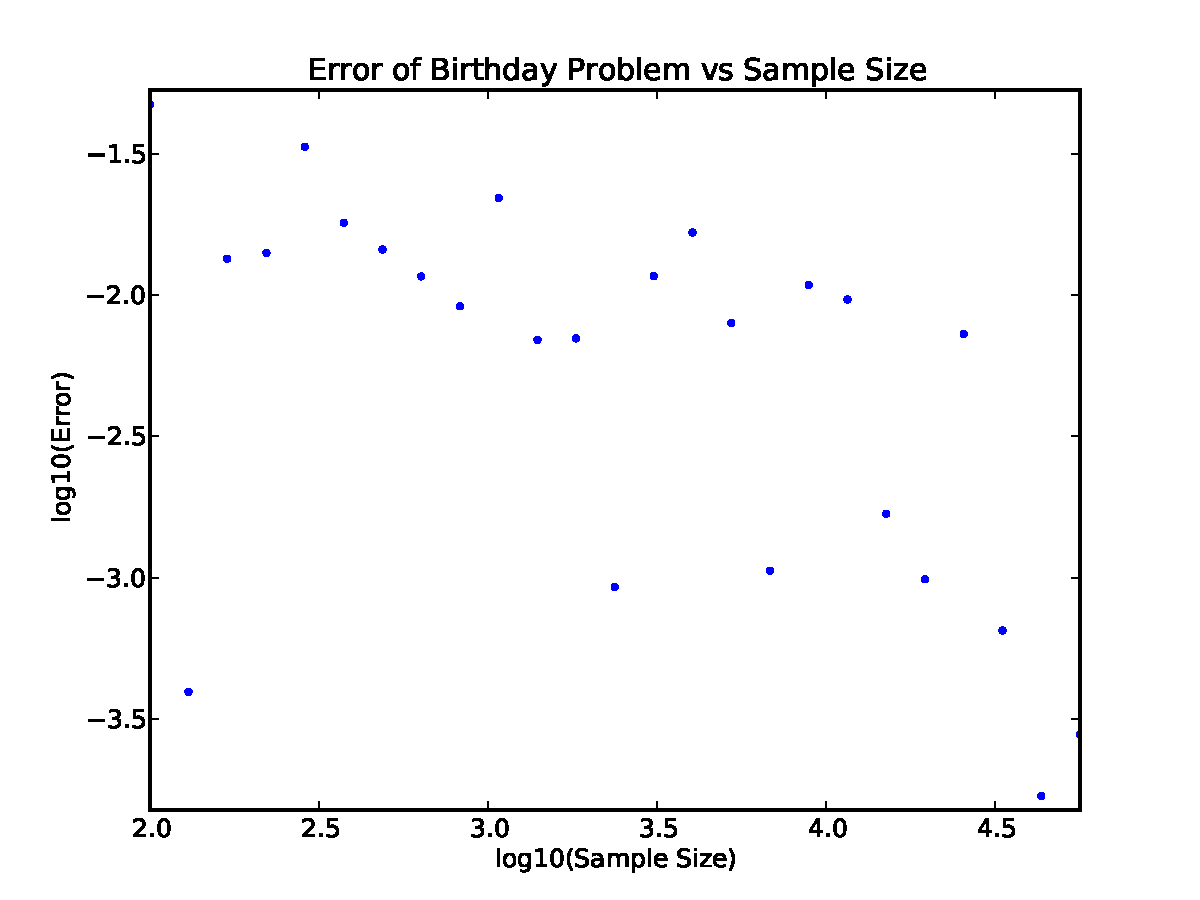
\includegraphics[width=0.8\textwidth]{birth_logerr_plot.pdf}
\caption{$\log_{10}$|error| vs $\log_{10} N$.}
\label{fig:birthplot2}
\end{figure} 

If there are N people, and 365 days, there are $ \frac{365!}{(365-N)!} $
ways for those N people to have unique birthdays (i.e. number of permuatations
of N distinct objects chosen from 365), and there are $365^N$ total ways to 
assign birthdays (unique or not) to N people. So, the probability of the N
people having unique birthdays is 
$$ \frac{365! / (365-N)!}{365^N}$$
which means the probability of at least two people having the same birthday
is just 1 minus that:
$$ 1 - \frac{365!}{365^{N}(365-N)!} $$

Now, plotting the error vs sample size 
(figures~\ref{fig:birthplot1} and \ref{fig:birthplot2})
we see, even though it isn't quite as clear as before, 
a convergence that goes as about $-1/2 \log N$ on the log-log plot, 
which means an actual convergence of $1/\sqrt{N}$.


\section{BONUS! More MC Integration! Only \$3.99 shipping and handling!}

We want to use hit-or-miss MC integration here to integrate $f(x) = x^2 + 1$ from 
$a = 2$ to $b = 3$, which is well described in the notes. The most important 
lines of code are 
\lstinputlisting[language=Python, firstline=40, lastline=41]{ws7.3.py}
Here, the array in the first line is made of True and False boolean values,
which are then summed over in the second line, giving the number of points
underneath the curve in the upper rectangle. Like in section 1, the sample sizes
were chosen to be evenly spaced on a logarithmic scale. Plotting the error vs the 
log of the sample size, we again see that the experiment converges. On the 
associated log-log plot, we see that it again converges as $1/\sqrt{N}$.

\begin{figure}[bth]
\centering
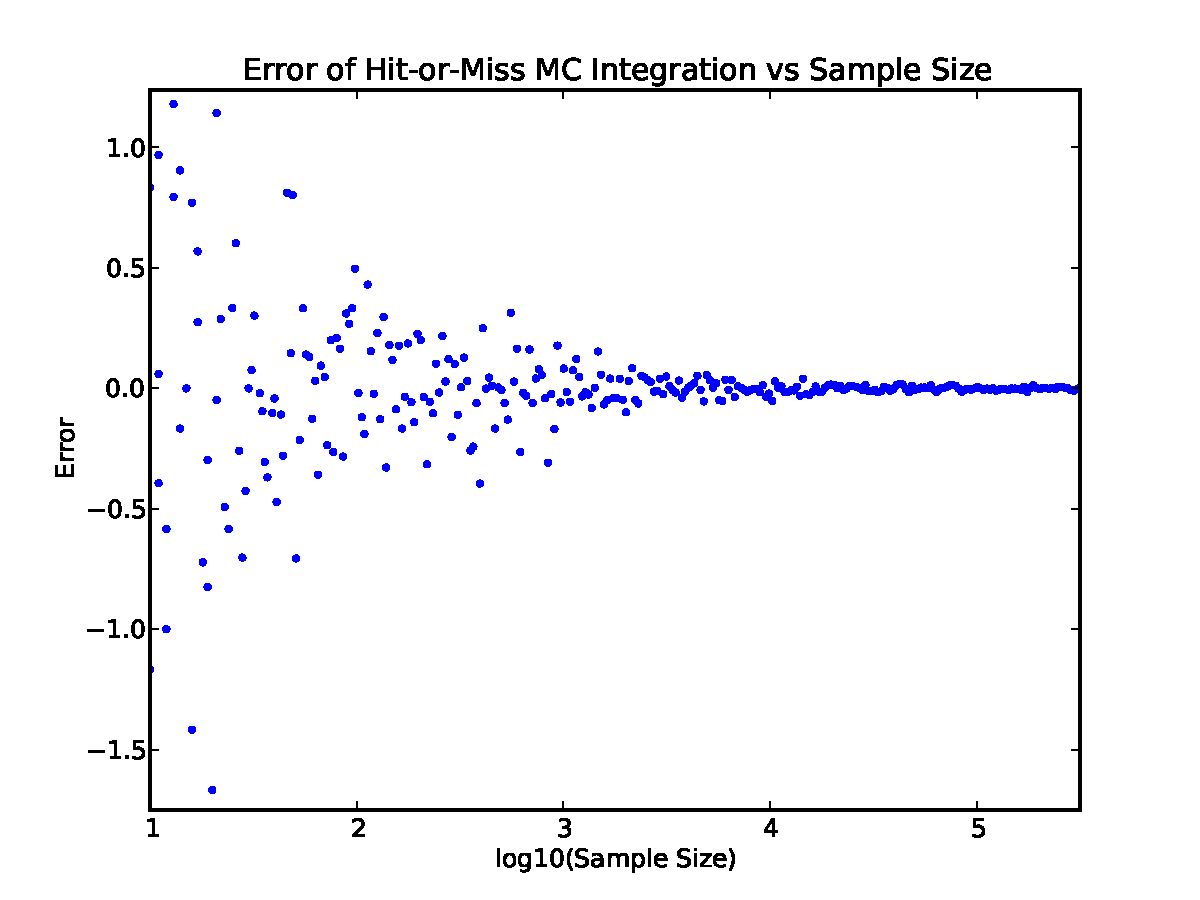
\includegraphics[width=0.8\textwidth]{MCint_err_plot.pdf}
\caption{Error of MC integration vs $\log_{10} N$.}
\label{fig:intplot1}
\end{figure}

\begin{figure}
\centering
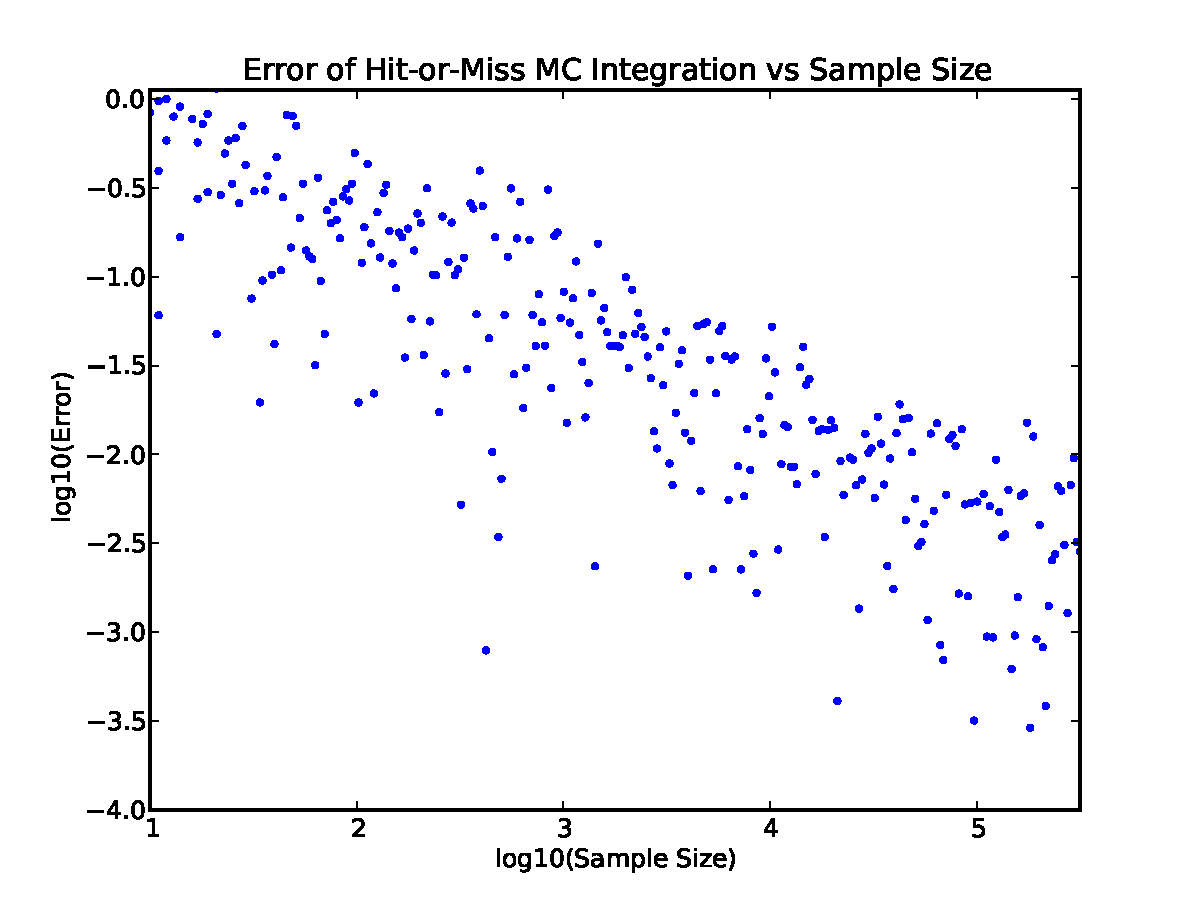
\includegraphics[width=0.8\textwidth]{MCint_logerr_plot.pdf}
\caption{$\log_{10}$|error| vs $\log_{10} N$.}
\label{fig:intplot2}
\end{figure} 


\end{document}
